% This file was created by matlab2tikz.
%
%The latest updates can be retrieved from
%  http://www.mathworks.com/matlabcentral/fileexchange/22022-matlab2tikz-matlab2tikz
%where you can also make suggestions and rate matlab2tikz.
%
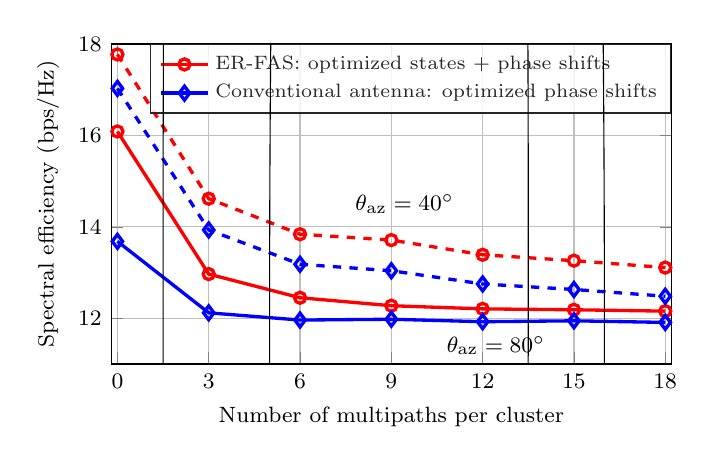
\begin{tikzpicture}[scale=1]

\begin{axis}[%
width=2.8in,
height=1.6in,
at={(0in,0in)},
scale only axis,
xmin=-0.2,
xmax=18.2,
xtick = {0,3,6,9,12,15,18},
xlabel style={font=\color{white!15!black},font=\footnotesize},
xticklabel style = {font=\color{white!15!black},font=\footnotesize},
xlabel={Number of multipaths per cluster},
ymin=11,
ymax=18,
ylabel style={font=\color{white!15!black},font=\footnotesize},
yticklabel style = {font=\color{white!15!black},font=\footnotesize},
ylabel={Spectral efficiency (bps/Hz)},
axis background/.style={fill=white},
xmajorgrids,
ymajorgrids,
legend style={at={(1,1)}, anchor=north east, font=\scriptsize, legend cell align=left, align=left, draw=white!15!black, fill opacity=0.85}
]
\addplot [color=red, line width=1.2pt, mark=o, mark options={solid, red}]
  table[row sep=crcr]{%
0	16.087390743277\\
3	12.9669627278226\\
6	12.4495852281104\\
9	12.2753091367489\\
12	12.2059641361206\\
15	12.1864293422317\\
18	12.1569004774112\\
};
\addlegendentry{\ac{ER-FAS}: optimized states + phase shifts}

\addplot [color=blue, line width=1.2pt, mark=diamond, mark options={solid, blue},mark size=2.5pt]
  table[row sep=crcr]{%
0	13.6829339650131\\
3	12.1195872950809\\
6	11.9614666732888\\
9	11.9791287537761\\
12	11.9252389244574\\
15	11.9448406312366\\
18	11.9098829011175\\
};
\addlegendentry{Conventional antenna: optimized phase shifts}

\addplot [color=red, dashed, line width=1.2pt, mark=o, mark options={solid, red}, forget plot]
  table[row sep=crcr]{%
0	17.7719594253263\\
3	14.6172110140971\\
6	13.8397487542046\\
9	13.7105935082057\\
12	13.3896920399889\\
15	13.2605223249006\\
18	13.1098718325458\\
};
\addplot [color=blue, dashed, line width=1.2pt, mark=diamond, mark options={solid, blue},mark size=2.5pt, forget plot]
  table[row sep=crcr]{%
0	17.0289547545375\\
3	13.9329371174651\\
6	13.1823217500994\\
9	13.0402743464238\\
12	12.7512325313032\\
15	12.6298635913446\\
18	12.4830501987156\\
};
\end{axis}

\begin{axis}[%
width=2.8in,
height=1.6in,
at={(0in,0in)},
scale only axis,
xmin=-0.2,
xmax=18.2,
ymin=11,
ymax=18,
axis line style={draw=none},
ticks=none,
axis x line*=bottom,
axis y line*=left
  ]
  \draw [black] (axis cs:7.5,13.5) ellipse [x radius=6, y radius=70];
  \node[right, align=left]
    at (axis cs:7.5,14.5) {\footnotesize{$\theta_\mathrm{az}=40^\circ$}};
  \draw [black] (axis cs:10.5,12.1) ellipse [x radius=5.5, y radius=50];
  \node[right, align=left]
    at (axis cs:10.5,11.4) {\footnotesize{$\theta_\mathrm{az}=80^\circ$}};
  \end{axis}
  
\end{tikzpicture}%